%\documentclass[mathserif]{beamer}
\documentclass[handout]{beamer}
%\usetheme{Goettingen}
\usetheme{Warsaw}
%\usetheme{Singapore}
%\usetheme{Frankfurt}
%\usetheme{Copenhagen}
%\usetheme{Szeged}
%\usetheme{Montpellier}
%\usetheme{CambridgeUS}
%\usecolortheme{}
%\setbeamercovered{transparent}
\usepackage[english, activeacute]{babel}
\usepackage[utf8]{inputenc}
\usepackage{amsmath, amssymb}
\usepackage{dsfont}
\usepackage{graphics}
\usepackage{cases}
\usepackage{graphicx}
\usepackage{pgf}
\usepackage{epsfig}
\usepackage{amssymb}
\usepackage{multirow}	
\usepackage{amstext}
\usepackage[ruled,vlined,lined]{algorithm2e}
\usepackage{amsmath}
\usepackage{epic}
\usepackage{epsfig}
\usepackage{fontenc}
\usepackage{framed,color}
\usepackage{palatino, url, multicol}
\usepackage{listings}
%\algsetup{indent=2em}


\vspace{-0.5cm}
\title{Introduction to Statistical Thinking}
\vspace{-0.5cm}
\author[Felipe Bravo Márquez]{\footnotesize
%\author{\footnotesize  
 \textcolor[rgb]{0.00,0.00,1.00}{Felipe José Bravo Márquez}} 
\date{ \today }




\begin{document}
\begin{frame}
\titlepage


\end{frame}


%%%%%%%%%%%%%%%%%%%%%%%%%%%


\begin{frame}{Introduction to Statistical Thinking}
\scriptsize{
\begin{itemize}
\item Statistical thinking is a systematic way of thinking about how we describe the \textbf{world} and use \textbf{data} to make decisions and predictions.

\item This is done taking into account the inherent \textbf{uncertainty} that exists in the real world.  \cite{poldrack2019statistical}

 
 \item The foundations of statistical thinking come primarily from mathematics and statistics, but also from computer science, psychology, and other fields of study. \cite{poldrack2019statistical}
 
 \item \textbf{Statistics}, in particular, is the discipline that concerns the collection, organization, analysis, interpretation, and presentation of data \cite{wiki:Statistics}.
 
\end{itemize}

\begin{figure}[h!]
	\centering
	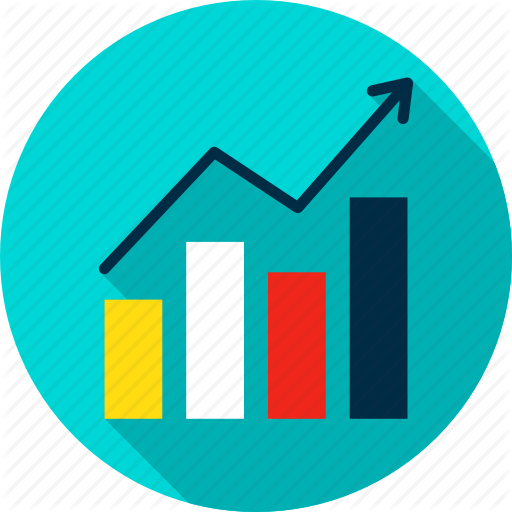
\includegraphics[scale=0.2]{pics/stats.png}
\end{figure}

} 
\footnotemark{These slides are mainly based on Chapter 1 of \cite{poldrack2019statistical}.}
\end{frame}



\begin{frame}{Statistical Thinking and Intuition}

\scriptsize{
\begin{itemize}
\item Human \textbf{intuition} often tries to answer the same questions that we can answer using statistical thinking, but often gets the answer \textbf{wrong}. 
\item For example, in recent years most Americans have reported that they think that violent crime was worse compared to the previous year (Pew Research Center). 
\item However, a statistical analysis of the actual crime data shows that in fact violent crime has steadily decreased since the 1990’s. 
\item Intuition fails us because we rely upon \textbf{best guesses} (which psychologists refer to as heuristics) that can often get it wrong. \cite{poldrack2019statistical}

\end{itemize}

}
 
\end{frame}





\begin{frame}{What can statistics do for us?}
There are three major things that we can do with statistics:

\begin{itemize}
\item \textbf{Describe}: The world is complex and we often need to describe it in a simplified way that we can understand.
\item \textbf{Decide}: We often need to make decisions based on data, usually in the face of uncertainty.
\item \textbf{Predict}: We often wish to make predictions about new situations based on our knowledge of previous situations.



\end{itemize}


 
\end{frame}



\begin{frame}{Example: Saturated Fat}

\scriptsize{
\begin{itemize}
\item Suppose we want to answer the following question: \\ Is saturated fat in our diet a bad thing?

\begin{figure}[h!]
	\centering
	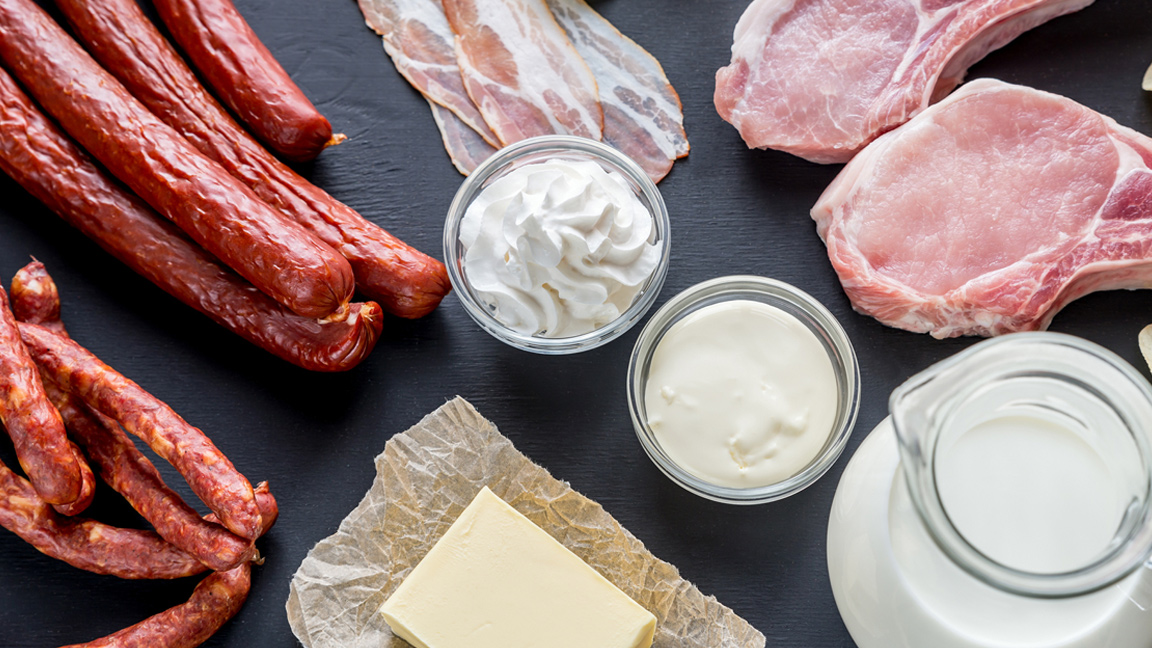
\includegraphics[scale=0.1]{pics/saturated-fat.jpg}
\end{figure}

\item Common sense approach: If we eat fat, then it's going to turn straight into fat in our bodies, right?
\item And we have all seen photos of arteries clogged with fat, so eating fat is going to clog our arteries, right?


\end{itemize}

}
 
\end{frame}



\begin{frame}{Example: Saturated Fat}

\scriptsize{
\begin{itemize}
\item Experts approach:  The Dietary Guidelines from the US Food and Drug Administration have as one of their Key Recommendations that ``A healthy eating pattern limits saturated fats''. 

\item You might hope that these guidelines would be based on good science, and in some cases they are.

\item However, as Nina Teicholz outlined in her book ``Big Fat Surprise'' \cite{teicholz2014big}, this particular recommendation seems to be based more on the dogma of nutrition researchers than on actual evidence. 

\begin{figure}[h!]
	\centering
	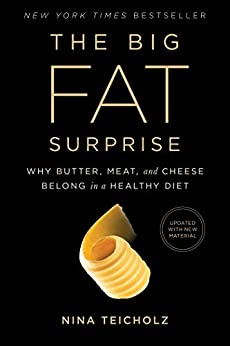
\includegraphics[scale=0.35]{pics/bigfat.jpg}
\end{figure}


\end{itemize}

}
 
\end{frame}


\begin{frame}{Example: Saturated Fat}

\scriptsize{
\begin{itemize}
\item Statistical approach:  we might look at actual scientific research.

\item PURE: a large study that has examined diets and health outcomes (including death) in more than 135,000 people from 18 different countries. 

\item One of the analyses of this dataset reported  how intake of various classes of macronutrients (including saturated fats and carbohydrates) was related to the likelihood of \textbf{dying} during the time that people were followed  \cite{dehghan2017associations}.

\item People were followed for a median of 7.4 years, meaning that half of the people in the study were followed for less and half were followed for more than 7.4 years. 


\end{itemize}

}
 
\end{frame}


\begin{frame}{Example: Saturated Fat}

\scriptsize{
\begin{itemize}
\item The following figure shows the relationship between the intake of both saturated fats and carbohydrates and the risk of dying from any cause.

\begin{figure}[h!]
	\centering
	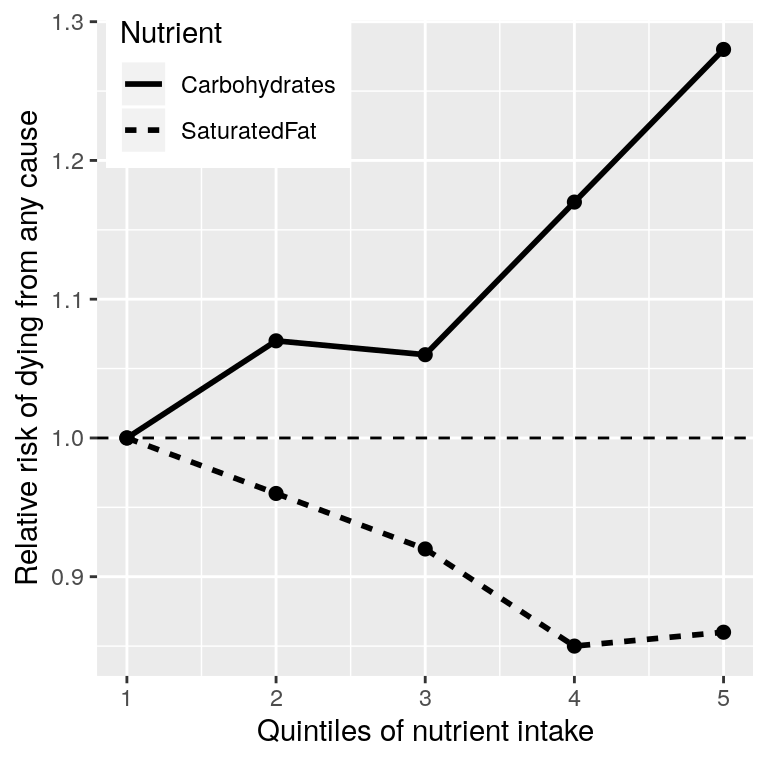
\includegraphics[scale=0.55]{pics/PureDeathSatFat-1.png}
\end{figure}


\item This plot is based on ten numbers.

\end{itemize}

}
 
\end{frame}


\begin{frame}{Example: Saturated Fat}

\scriptsize{
\begin{itemize}
\item To obtain these numbers, the researchers split the group of 135,335 study participants (which we call the ``sample'') into 5 groups (“quintiles”).
\item The first quintile contains the 20\% of people with the lowest intake, and the 5th quintile contains the 20\% with the highest intake. 
\item The researchers then computed how often people in each of those groups died during the time they were being followed. 
\item The figure expresses this in terms of the relative risk of dying in comparison to the lowest quintile.
\item If this number is greater than one, it means that people in the group are more likely to die than are people in the lowest quintile.
\item Whereas if it’s less than one, it means that people in the group are less likely to die. 
\end{itemize}

}
 
\end{frame}


\begin{frame}{Example: Saturated Fat}

\scriptsize{
\begin{itemize}
\item The figure is pretty clear: People who ate more saturated fat were less likely to die during the study.
\item The opposite is seen for carbohydrates: the more carbs a person ate, the more likely they were to die during the study. \item This example shows how we can use statistics to describe a complex dataset in terms of a much simpler set of numbers.
\item If we had to look at the data from each of the study participants at the same time, we would be overloaded with data. 
\item It would also be hard to see the pattern that emerges when they are described more simply.

\end{itemize}

}
 
\end{frame}

\begin{frame}{Example: Saturated Fat}

\scriptsize{
\begin{itemize}
\item Despite the figures in the figure, we also know that there is a lot of \textbf{uncertainty} in the data.
\item There are some people who died early even though they ate a low-carb diet, and, other people who ate a ton of carbs but lived to a ripe old age. 
\item Given this variability, we want to decide whether the relationships that we see in the data are large enough that we wouldn't expect them to occur \textbf{randomly}.
\item Statistics provide us with the tools to make these kinds of decisions.
\item Often people from the outside view this as the \textbf{main purpose} of statistics. 
\item But as we will see throughout the course, this need for \textbf{black-and-white} decisions based on fuzzy evidence has often led researchers down the wrong path.
\end{itemize}

}
 
\end{frame}


\begin{frame}{Example: Saturated Fat}

\scriptsize{
\begin{itemize}
\item If our conclusions were limited to the specific people in the study at a particular time, then the study would not be very useful. 
\item Based on the data we would also like to make \textbf{predictions} about future outcomes. 
\item For example, a life insurance company might want to use data about a particular person's intake of fat and carbohydrate to predict how long they are likely to live.
\item An important aspect of prediction is that it requires us to \textbf{generalize} from the data we already have to some other situation, often in the future.
\item In general, researchers must assume that their particular sample is \textbf{representative} of a larger \textbf{population}.
\item This requires that they obtain the sample in a way that provides an \textbf{unbiased} picture of the population. 
\item For example, if the PURE study had only recruited vegetarian participants, we would probably not want to generalize the results to non-vegetarians.
\end{itemize}

}
 
\end{frame}

\begin{frame}{The big ideas of statistics}

\scriptsize{
There are a number of very basic ideas that cut through nearly all aspects of statistical thinking. 

\begin{enumerate}
 \item Learning from data
 \item Aggregation
 \item Uncertainty
 \item Sampling from a population
 \item Causality and statistics
\end{enumerate}

Next, we examine each of them in more detail.

}
 
\end{frame}


\begin{frame}{Learning from data}

\scriptsize{
\begin{itemize}
\item One way to think of statistics is as a set of tools that enable us to learn from data.\footnote{As you may have realized statistics is closely related to machine learning.}
\item In any situation, we start with a set of ideas or hypotheses about what might be the case. 
\item In the PURE study, the researchers may have started out with the expectation that eating more fat would lead to higher death rates, given the prevailing negative dogma about saturated fats. 
\item Later in the course we will introduce the idea of prior knowledge, which is meant to reflect the knowledge that we bring to a situation. 

\item Statistics provides us with a way to describe how new data can be best used to update our beliefs.
\end{itemize}

}
 
\end{frame}


\begin{frame}{Aggregation}

\scriptsize{
\begin{itemize}
\item Another way to think of statistics is as ``the science of throwing away data''.
\item In the example of the PURE study above, we took more than 100,000 numbers and condensed them into ten. 
\item It is this kind of aggregation that is one of the most important concepts in statistics. 
\item Statistics provides us ways to characterize the structure of aggregates of data, and with theoretical foundations that explain why this usually works well.
\item However, it’s also important to keep in mind that aggregation can go too far.
\item Sometimes, a summary can provide a misleading picture of the data.
\end{itemize}

}
 
\end{frame}


\begin{frame}{Uncertainty}

\scriptsize{
\begin{itemize}
\item The world is an uncertain place.
\item We now know that cigarette smoking causes lung cancer, but this causation is probabilistic.
\item A 68-year-old man who smoked two packs a day for the past 50 years and continues to smoke has a 15\% risk of getting lung cancer.
\item This is much higher than the chance of lung cancer in a nonsmoker. 
\item However, it also means that there will be many people who smoke their entire lives and never get lung cancer. 
\end{itemize}

}
 
\end{frame}


\begin{frame}{Uncertainty}

\scriptsize{
\begin{itemize}
\item Statistics provides us with the tools to characterize uncertainty, to make decisions under uncertainty, and to make predictions whose uncertainty we can quantify.

\item One often sees journalists write that scientific researchers have ``proven'' some hypothesis. 
\item But statistical analysis can never ``prove'' a hypothesis, in the sense of demonstrating that it must be true.
\item Statistics can provide us with evidence, but it's always tentative and subject to the uncertainty that is always present in the real world.
\end{itemize}
}
 
\end{frame}


\begin{frame}{Sampling from a population}

\scriptsize{
\begin{itemize}
\item The concept of aggregation implies that we can make useful insights by collapsing across data.
\item But how much data do we need? 
\item The idea of sampling says that we can summarize an entire population based on just a small number of samples from the population.
\item As long as those samples are obtained in the right way. 
\end{itemize}

}

\begin{figure}[h!]
	\centering
	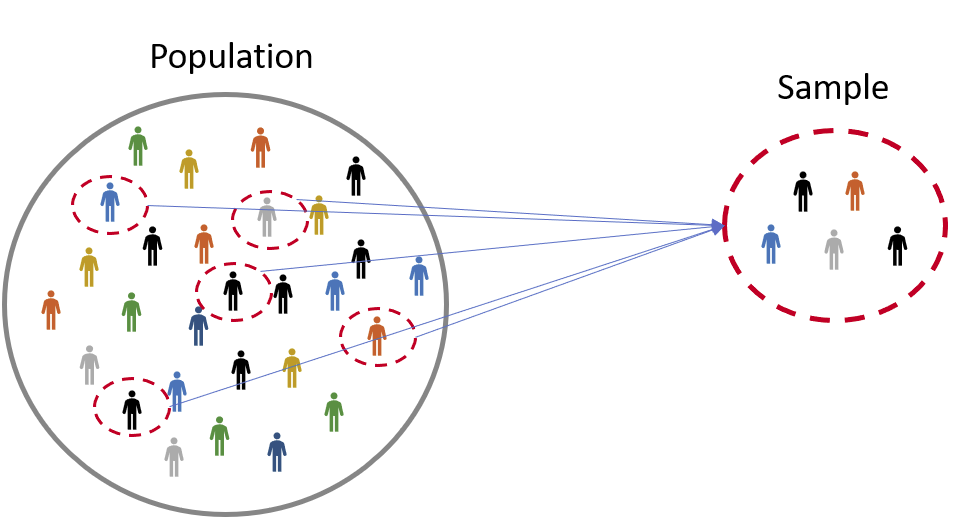
\includegraphics[scale=0.3]{pics/sampling.png}
\end{figure}
 
\end{frame}


\begin{frame}{Sampling from a population}

\scriptsize{
\begin{itemize}
\item For example, the PURE study enrolled a sample of about 135,000 people.
\item But its goal was to provide insights about the billions of humans who make up the population from which those people were sampled. 
\item The way that the study sample is obtained is critical, as it determines how broadly we can generalize the results.
\item Another fundamental insight about sampling is that while larger samples are always better (in terms of their ability to accurately represent the entire population), there are diminishing returns as the sample gets larger. 

\item In fact, the rate at which the benefit of larger samples decreases follows a simple mathematical rule, growing as the square root of the sample size.
\item Such that in order to double the quality of our data we need to quadruple the size of our sample.
\end{itemize}

}

 
\end{frame}


\begin{frame}{Causality and statistics}

\scriptsize{
\begin{itemize}
\item The PURE study seemed to provide pretty strong evidence for a positive relationship between eating saturated fat and living longer.
\item However, this doesn't tell us what we really want to know: If we eat more saturated fat, will that cause us to live longer?
\item This is because we don't know whether there is a direct causal relationship between eating saturated fat and living longer. 
\item The data are consistent with such a relationship, but they are equally consistent with some other factor causing both higher saturated fat and longer life.

\end{itemize}

\begin{figure}[h!]
	\centering
	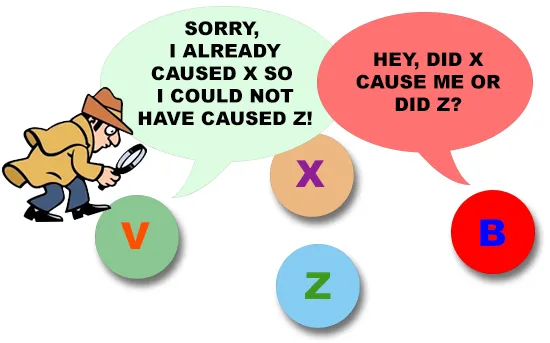
\includegraphics[scale=0.4]{pics/causality.png}
\end{figure}

}
 
\end{frame}



\begin{frame}{Causality and statistics}

\scriptsize{
\begin{itemize}
\item For example, it is likely that people who are richer eat more saturated fat and richer people tend to live longer.
\item Their longer life is not necessarily due to fat intake though.
\item It could instead be due to better health care, reduced psychological stress, better food quality, or many other factors. 
\item The PURE study investigators tried to account for these factors.
\item But we can't be certain that their efforts completely removed the effects of other variables. 
\item The fact that other factors may explain the relationship between saturated fat intake and death is an example of the claim  that ``correlation does not imply causation''.
\end{itemize}

}
 
\end{frame}




\begin{frame}{Causality and statistics}

\scriptsize{
\begin{itemize}
\item Although observational research (like the PURE study) cannot conclusively demonstrate causal relations, we generally think that causation can be demonstrated using studies that experimentally control and manipulate a specific factor.

\item In medicine, such a study is referred to as a randomized controlled trial (RCT).
\item Let’s say that we wanted to do an RCT to examine whether increasing saturated fat intake increases life span. 
\item To do this, we would sample a group of people, and then assign them to either a treatment group or a control group.
\item Treatment group: people told to increase their saturated fat intake.
\item  Control group: people told to keep eating the same as before. 
\end{itemize}

}
 
\end{frame}


\begin{frame}{Causality and statistics}

\scriptsize{
\begin{itemize}
\item It is essential that we assign the individuals to these groups randomly. 
\item Otherwise, people who choose the treatment might be different in some way than people who choose the control group.
\item For example, they might be more likely to engage in other healthy behaviors as well. 
\item We would then follow the participants over time and see how many people in each group died. 
\item Because we randomized the participants to treatment or control groups, we can be reasonably confident that there are no other differences between the groups that would confound the treatment effect.
\item However, we still can’t be certain because sometimes randomization yields treatment versus control groups that do vary in some important way.
\end{itemize}

}
 
\end{frame}


\begin{frame}{Causality and statistics}

\scriptsize{
\begin{itemize}
\item Researchers often try to address these confounds using statistical analyses, but removing the influence of a confound from the data can be very difficult.
\item A number of RCTs have examined the question of whether changing saturated fat intake results in better health and longer life. 
\item These trials have focused on reducing saturated fat because of the strong dogma amongst nutrition researchers that saturated fat is deadly.
\item Most of these researchers would have probably argued that it was not ethical to cause people to eat more saturated fat! \item However, the RCTs have shown a very consistent pattern: Overall there is no appreciable effect on death rates of reducing saturated fat intake.
\end{itemize}

}
 
\end{frame}



\begin{frame}{Course Philosophy}

\scriptsize{
There two radical approaches to teach an introductory course on statistics.
\begin{block}{Mathematical Statistics}
 \begin{itemize}
\item This is usually taught in mathematics departments.
\item The focus is on the mathematical aspects of statistics (e.g., asymptotic properties).
\end{itemize}
\end{block}


\begin{block}{Applied Statistics}
 \begin{itemize}
\item This is usually taught in health and social science departments (e.g., psychology).
\item The focus in on the methods (e.g., t-test, ANOVA, linear regression) and how to apply them to the specific field.
\end{itemize}
\end{block}




}
 
\end{frame}

\begin{frame}{Course Philosophy}

\scriptsize{
 \begin{itemize}
\item In my personal opinion mathematical courses are in many cases hard to grasp for non-mathematical students and don't pay enough attention to the use of statistics in real world problems.
\item On the other hand, applied courses sometimes omit the fundamental assumptions on which the methods are based and end up being a kind of recipe book of methods for ad hoc problems. 

\item This course attempts to bring a balance between both paradigms.

\item We will reflect and discuss the fundamental assumptions and ideas on which statistical models are based (without going too deeply into the mathematics). 

\item We will be aware at all times that no method or tool fits all problems perfectly, or as it is commonly said: ``all models are wrong but some are useful''.

\item  Finally, we will discuss thoroughly the two major schools of statistical inference: \textbf{frequentist} and \textbf{Bayesian}.

\end{itemize}



}
 
\end{frame}


\begin{frame}{Example of flowchart (recipe book) taken from \cite{mcelreath2020statistical}} 


\begin{figure}[h!]
	\centering
	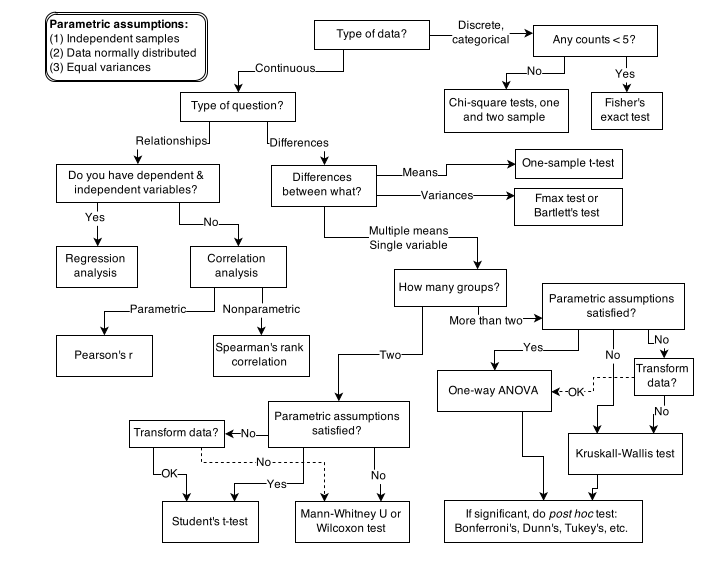
\includegraphics[scale=0.38]{pics/flowchart.png}
\end{figure}


 
\end{frame}

\begin{frame}{Roadmap}

\scriptsize{
The main topics that will be covered in this course are:
\begin{itemize}
\item Foundations
\begin{itemize}\scriptsize{
\item Statistical Programming in R
\item Descriptive Statistics
\item Probability}
\end{itemize}
\item Frequentist Inference
\begin{itemize}\scriptsize{
\item Point Estimators
\item Confidence Intervals
\item Hypothesis Testing
\item Linear Regression}
\end{itemize}
\item Bayesian Inference
\begin{itemize}\scriptsize{
\item Posterior Distributions
\item Point and Interval Bayesian Estimates
\item Bayesian Linear Regression
\item Markov Chain Montecarlo}
\end{itemize}
\item Other Topics
\begin{itemize}\scriptsize{
\item Model Evaluation using Information Criteria
\item Graphical Models
\item Multi-level Models}
\end{itemize}
\end{itemize}

}
 
\end{frame}


%%%%%%%%%%%%%%%%%%%%%%%%%%%
\begin{frame}[allowframebreaks]\scriptsize
\frametitle{References}
\bibliography{bio}
\bibliographystyle{apalike}
%\bibliographystyle{flexbib}
\end{frame}  









%%%%%%%%%%%%%%%%%%%%%%%%%%%

\end{document}
